\item \textbf{Compresión del contexto del sistema}

\begin{itemize}

          \item ADMINISTRAR — Gerente $\leftrightarrow$ Sucursal — 1:1
          
Gerente: total (1,1)

Sucursal: parcial (0,1)

          \item PERTENECE — Máquina $\leftrightarrow$ Sucursal — N:1
          
Máquina: total (1,1)

Sucursal: parcial (0,N)

          \item CONTENER — Máquina $\leftrightarrow$ Juego — N:1
          
Máquina: total (1,1)

Juego: parcial (0,N)


          \item TENER — Cliente $\leftrightarrow$ Tarjeta — 1:1
          
Cliente: total (1,1)

Tarjeta: total (1,1)

          \item EMITIR — Cajero $\leftrightarrow$ Tarjeta — 1:N
          
Cajero: parcial (0,N)

Tarjeta: total (1,1)

          \item EFECTUAR — Sucursal $\leftrightarrow$ Recarga — 1:N
          
Sucursal: parcial (0,N)

Recarga: total (1,1)

          \item RECIBIR — Tarjeta $\leftrightarrow$ Recarga — 1:N
          
Tarjeta: parcial (0,N)

Recarga: total (1,1)

          \item PROCESAR — Cajero $\leftrightarrow$ Recarga — 1:N
          
Cajero: parcial (0,N)

Recarga: total (1,1)

          \item OCURRIR — Máquina $\leftrightarrow$ Partida — 1:N
          
Máquina: parcial (0,N)

Partida: total (1,1)

          \item REGISTRAR — Tarjeta $\leftrightarrow$ Partida — 1:N
          
Tarjeta: parcial (0,N)

Partida: total (1,1)

          \item SOLICITAR — Cliente $\leftrightarrow$ Canje — 1:N
          
Cliente: parcial (0,N)

Canje: total (1,1)

          \item INCLUIR — Premio $\leftrightarrow$ Canje — 1:N
          
Premio: parcial (0,N)

Canje: total (1,1)

          \item PROCESAR — EncargadoDePremios $\leftrightarrow$ Canje — 1:N
          
EncargadoDePremios: parcial (0,N)

Canje: total (1,1)

          \item OCURRIR — Sucursal $\leftrightarrow$ Canje — 1:N
          
Sucursal: parcial (0,N)

Canje: total (1,1)

          \item REALIZAR — Técnico $\leftrightarrow$ Mantenimiento — 1:N
          
Técnico: parcial (0,N)

Mantenimiento: total (1,1)

          \item RECIBIR — Máquina $\leftrightarrow$ Mantenimiento — 1:N
          
Máquina: parcial (0,N)

Mantenimiento: total (1,1)

          \item REGISTRAR — Sucursal $\leftrightarrow$ Inventario — 1:N
          
Sucursal: parcial (0,N)

Inventario: total (1,1)

          \item CONTENER — Premio $\leftrightarrow$ Inventario — 1:N
          
Premio: parcial (0,N)

Inventario: total (1,1)

            \item \textbf{Herencia}

\textbf{SuperEntidad:} Empleado.

Completez: total.

Restricción disyuntiva: Disyunción.

\textbf{SubEntidades:}

Cajero.
Gerente.
Técnico.
Encargado de premios.

\end{itemize}

\begin{figure}[htbp]
    \centering
    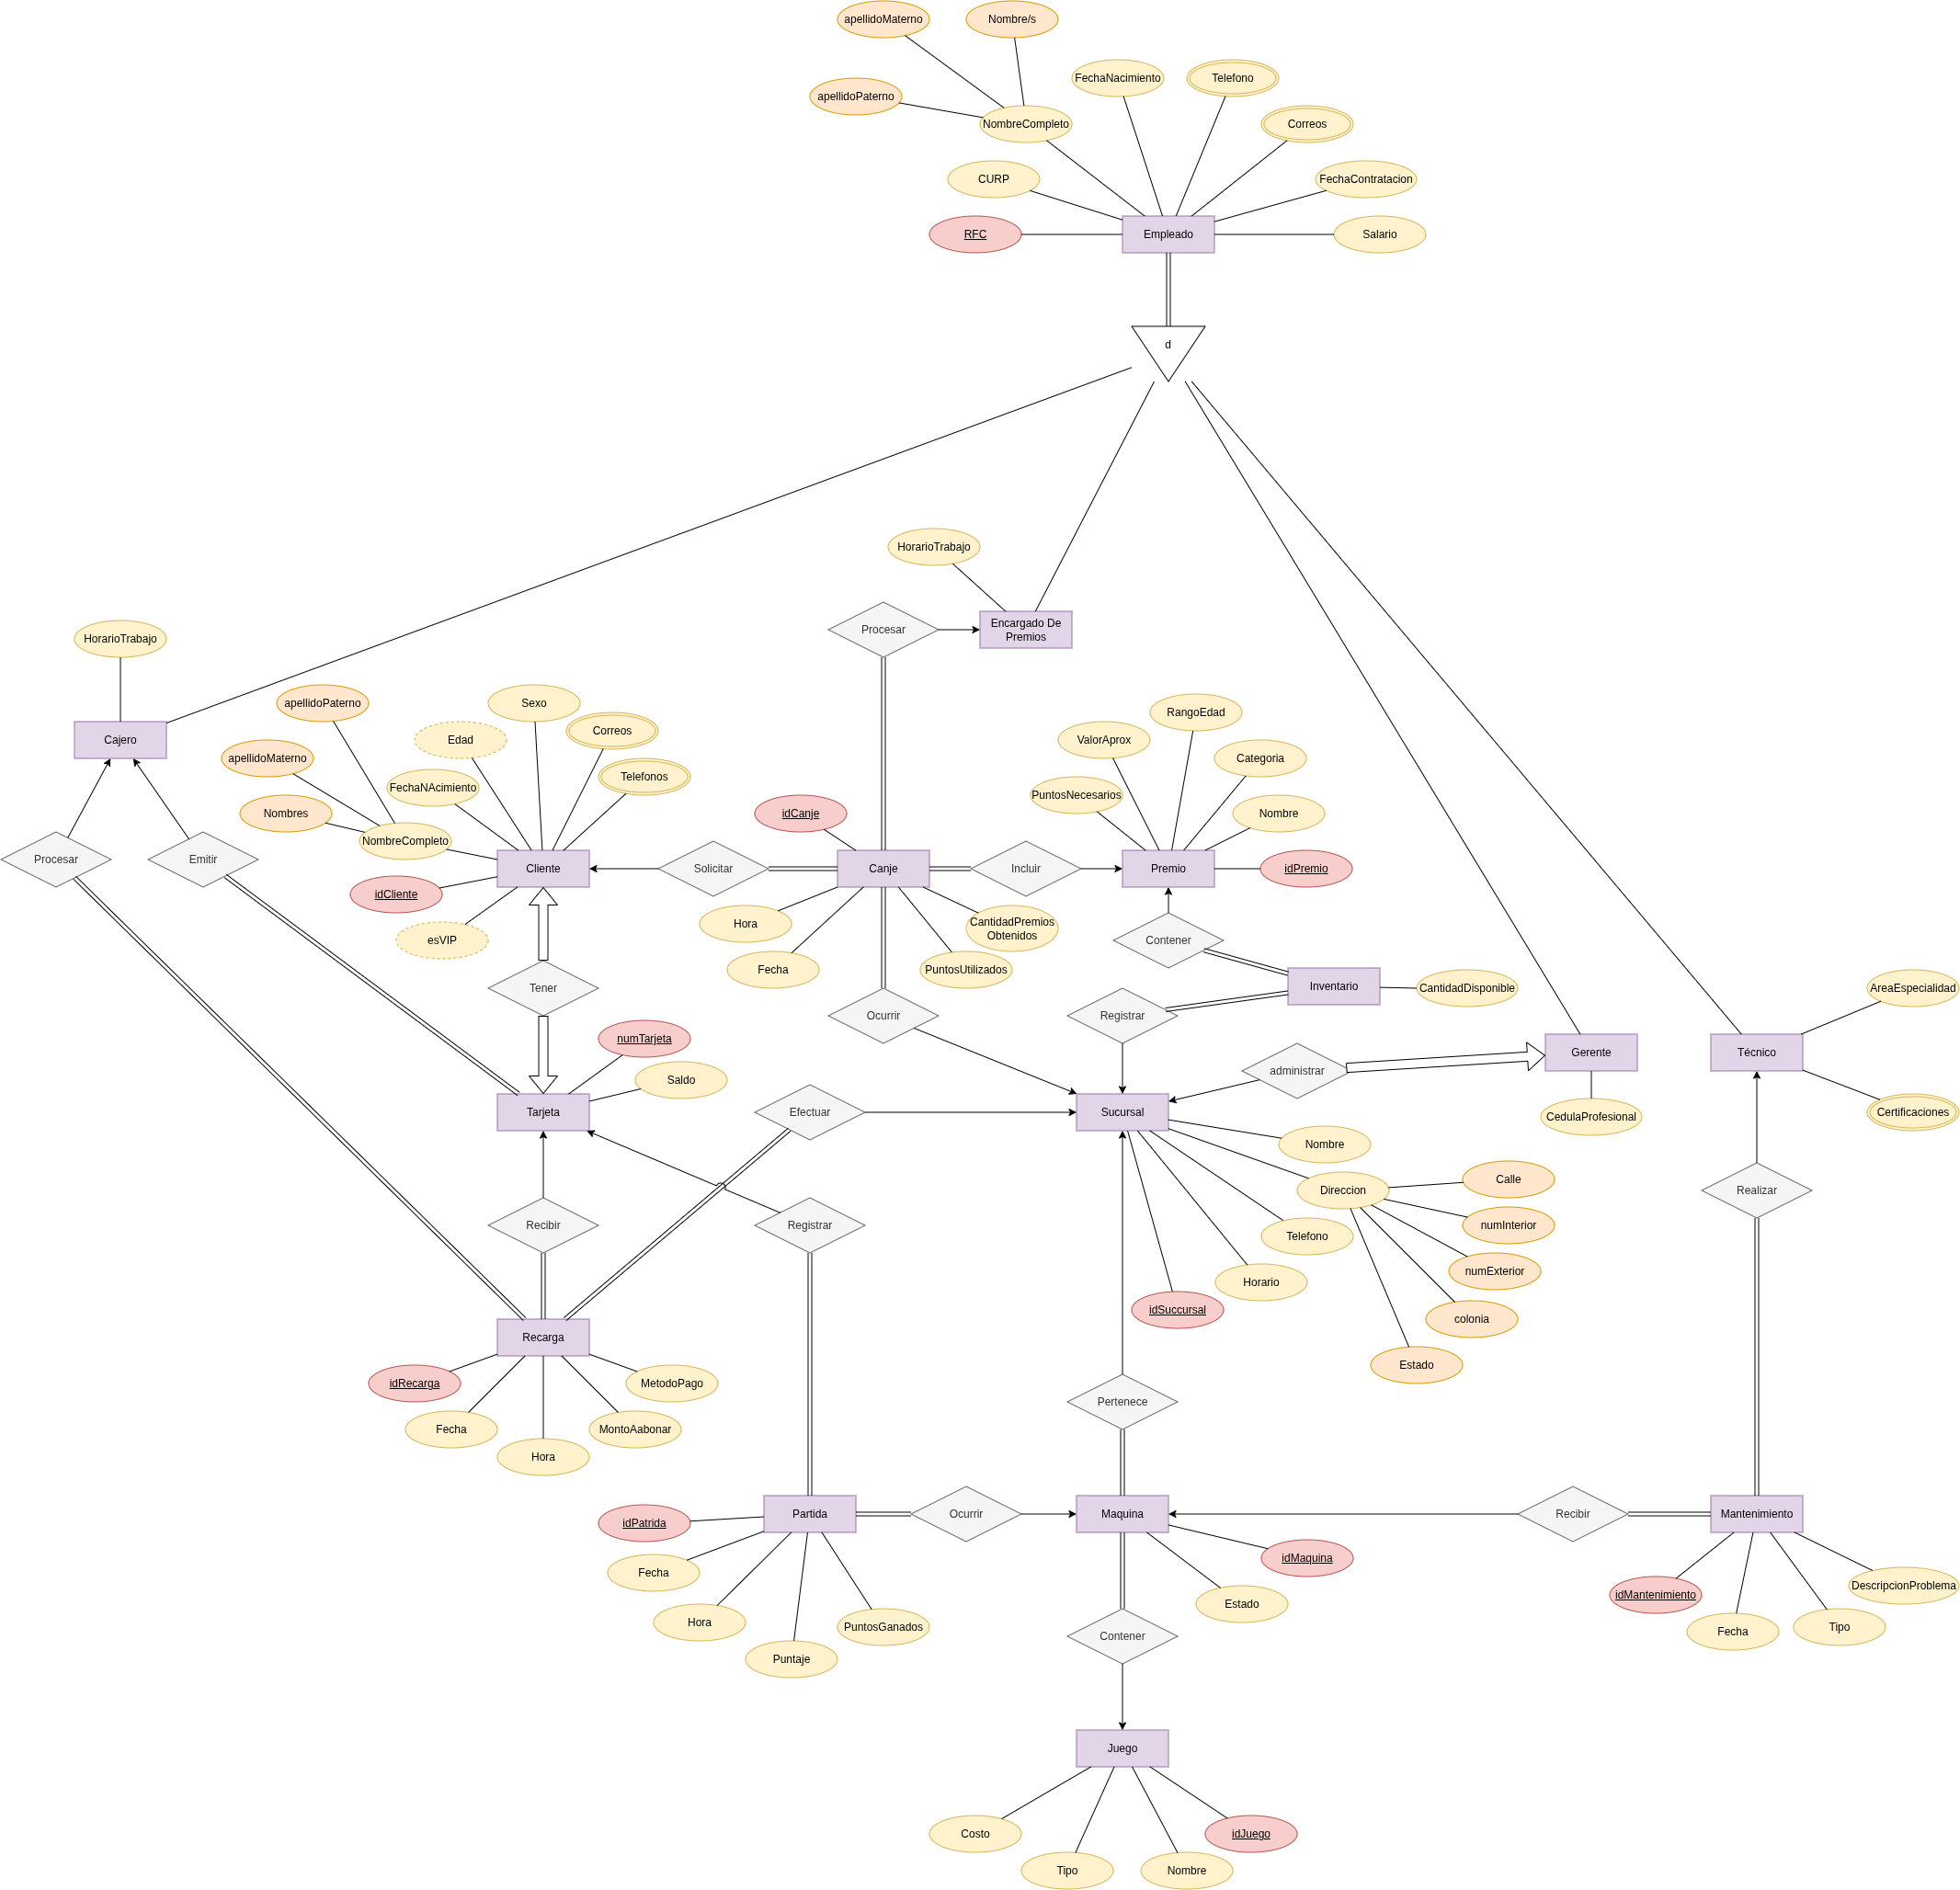
\includegraphics[width=0.7\textwidth]{Diagramas/diagramaPractica02.drawio.png}
    \caption{Diagrama}
    \label{fig:etiqueta_imagen}
\end{figure}

\newpage
